\chapter{من الجسيمات إلى حقل كمي بسيط}

لنبنِ الحقل الكمي البسيط مرة أخرى، ولكن من زاوية مختلفة قليلًا. هناك طريقان إلى نظرية الحقل الكمي. يمكننا أن نبدأ بالجسيمات ونكتشف لماذا يكون الحقل هو اللغة الطبيعية لها، أو أن نبدأ بحقل موجي ونكتشف لماذا تأتي إثاراته على هيئة كمّات. كلا الطريقين مفيد. وهنا سنبقى في الطريق الأول.

يمكن لميكانيكا الكم العادية أن تصف جسيمًا واحدًا، أو جسيمين، أو أي عدد ثابت آخر. لكن الطبيعة لا تلتزم بذلك القيد. يتغير عدد الفوتونات في غرفة كلما أطلقت الأضواء إشعاعًا أو امتصته. وتضمحل الجسيمات غير المستقرة. ففي اضمحلال بيتا مثلًا،
\begin{equation}
n\longrightarrow p+e^-+\bar{\nu}_e,
\end{equation}
ولذلك تتغير أعداد عدة أنواع من الجسيمات دفعة واحدة. ومن ثم نريد ميكانيكا كم واحدة تتسع لاحتواء كل عدد إشغال ممكن، وأن تحتوي في نهاية المطاف العمليات التي تنقل النظام من بعضها إلى بعض.

في الوقت الحاضر سنبسّط تبسيطًا شديدًا. هناك نوع واحد من الجسيمات غير النسبية. سنوسّع أولًا فضاء حالاته بحيث يمكنه أن يستوعب أي عدد من الجسيمات، وبعد ذلك فقط نناقش أنواعًا أكثر، والنسبية، والتشتت، والاضمحلال. ليست الرياضيات هنا صعبة على نحو خاص، لكن تغيّر المنظور تجريدي. ومن المفيد أن نأخذ الخطوات ببطء كافٍ بحيث لا تحجب الرموز الفكرة.

\section{نقطة البدء: الجسيم الواحد}

لنبدأ بجسيم مفرد في الحالة \(|\psi\rangle\). دالته الموجية في فضاء الموضع هي
\begin{equation}
\psi(x)=\langle x|\psi\rangle.
\label{eq:l07-wavefunction}
\end{equation}
وهذا الرمز الصغير \(\psi\) هو دالة عادية ذات قيم عقدية. وليس بعدُ حقلًا كميًا، وليس مؤثرًا على فضاء حالات متعدد الجسيمات.

تقول قاعدة بورن إن
\begin{equation}
\rho_\psi(x)=|\psi(x)|^2=\psi^*(x)\psi(x)
\label{eq:l07-born-density}
\end{equation}
هي كثافة الاحتمال لإيجاد الجسيم عند \(x\). وبالنسبة إلى حالة مطبَّعة،
\begin{equation}
\int dx\,\psi^*(x)\psi(x)=1.
\label{eq:l07-one-particle-normalization}
\end{equation}
فالطرف الأيمن هو الاحتمال الكلي. وبما أن هذه المسألة تحتوي جسيمًا واحدًا بالضبط، فإنه يساوي أيضًا عدد الجسيمات. وستصبح هذه المصادفة قرينة مفيدة، مع أنها هنا أمر بديهي.

\begin{classroomqa}
\lecturetimestamp{00:09:13}
\audiencequestion{لماذا يجب أن تكون كثافة الاحتمال على الصورة \(\psi^*(x)\psi(x)\)؟}
\lecturerresponse{هذه هي قاعدة بورن، وهي إحدى مسلَّمات ميكانيكا الكم. سعة ناتج الموضع \(x\) هي \(\langle x|\psi\rangle\)؛ وكثافة الاحتمال هي مربع القيمة المطلقة لهذه السعة. وهي لا تُستنبط من البناء الحقلي المستخدم لاحقًا.}
\end{classroomqa}

\section{الأنماط، والتعامد، والاكتمال}

هناك أسس كثيرة مفيدة لفضاء هيلبرت ذي الجسيم الواحد. وتشكل الحالات الذاتية للموضع أحد هذه الأسس. كما تشكل الحالات الذاتية لأي مؤثر هيرميتي أساسًا آخر، مع التحفظات المعتادة المتعلقة بالانحلال والأطياف المستمرة. وبما أن الطاقة ستغدو مهمة بعد قليل، فلنختر مجموعة تامة متعامدة معياريًا من الحالات الذاتية لطاقة الجسيم الواحد
\begin{equation}
|1\rangle,\ |2\rangle,\ldots,
\qquad
\psi_i(x)=\langle x|i\rangle.
\end{equation}

يجعل مثال الجسيم في صندوق الفهرس \(i\) شيئًا ملموسًا. فالدالة الموجية للحالة القاعية لا تحتوي على عقدة داخلية، وتحتوي الحالة التالية على عقدة واحدة، أما الحالات الأعلى فتتذبذب بسرعة أكبر. وهي في الأساس موجات جيبية في بئر مربعة لا نهائية مثالية.

\begin{figure}[htbp]
\centering
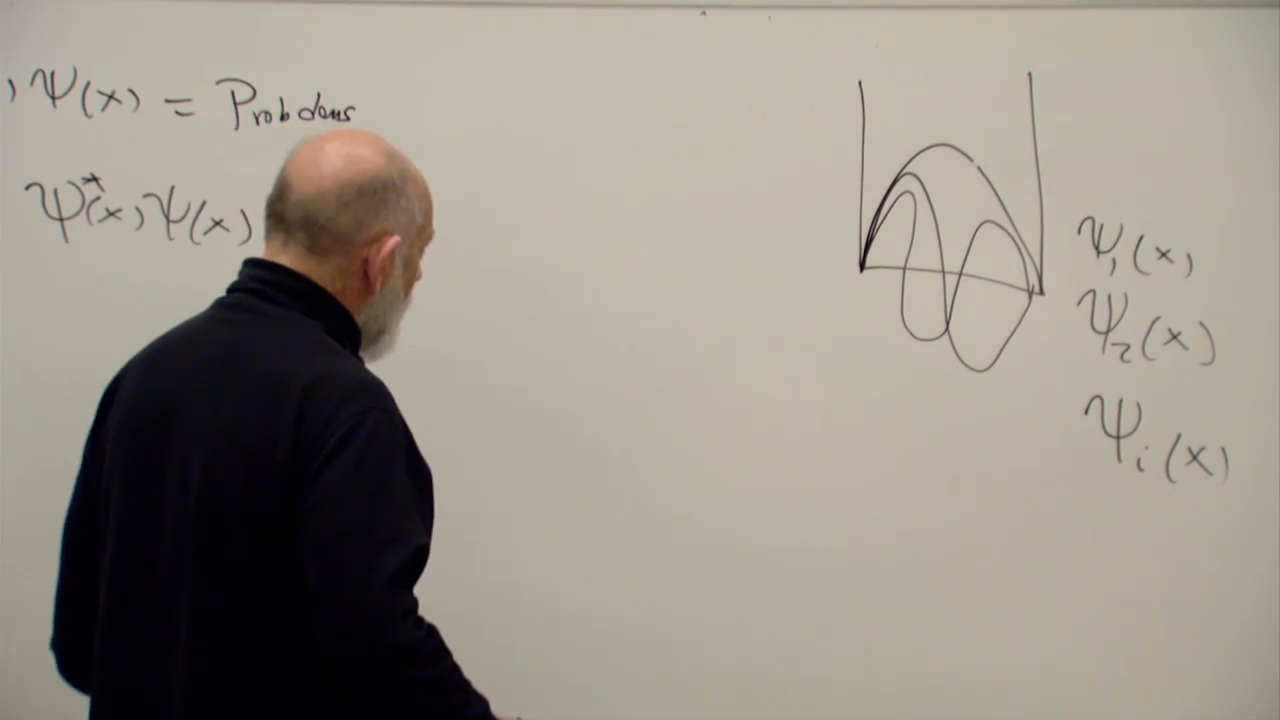
\includegraphics[width=0.94\linewidth]{lecture_07_frame_01.png}
\caption{أنماط الصندوق على لوحة المحاضرة. والآثار المتبقية في اليسار هي كثافة بورن وتطبيع الجسيم الواحد؛ أما البئر في اليمين فتُظهر \(\psi_1(x)\) و\(\psi_2(x)\) والوسم العام \(\psi_i(x)\).}
\lectureframe{00:08:25}
\end{figure}

يمكن فصل بنية الأنماط نفسها عن الحجب الموجود على اللوح أثناء الشرح:
\begin{figure}[htbp]
\centering
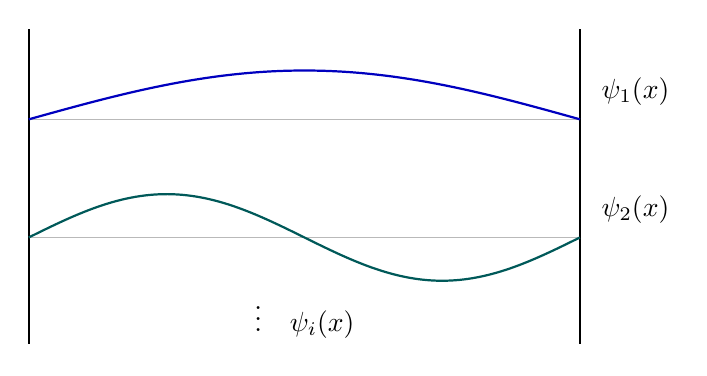
\begin{tikzpicture}[x=1cm,y=1cm]
  \draw[thick] (0,0) -- (0,4.0);
  \draw[thick] (7,0) -- (7,4.0);
  \draw[gray!55] (0,2.85) -- (7,2.85);
  \draw[gray!55] (0,1.35) -- (7,1.35);
  \draw[blue!75!black,thick,domain=0:7,samples=120]
    plot (\x,{2.85+0.62*sin(180*\x/7)});
  \draw[teal!70!black,thick,domain=0:7,samples=120]
    plot (\x,{1.35+0.55*sin(360*\x/7)});
  \node[right] at (7.15,3.20) {$\psi_1(x)$};
  \node[right] at (7.15,1.70) {$\psi_2(x)$};
  \node at (3.5,0.38) {$\vdots\quad\psi_i(x)$};
\end{tikzpicture}
\caption{إعادة بناء نظيفة للرسم التخطيطي الكيفي للصندوق. والإزاحات العمودية لا تفعل إلا فصل الدالتين الموجيتين لأغراض العرض.}
\end{figure}

التعامد المعياري هو
\begin{equation}
\int dx\,\psi_i^*(x)\psi_j(x)=\delta_{ij}.
\label{eq:l07-orthonormality}
\end{equation}
فإذا كان \(i=j\) كانت الحالة مطبَّعة ويكون التكامل واحدًا. وإذا كان \(i\ne j\) كانت الحالتان متعامدتين وينعدم التكامل.

والاكتمال هو العبارة التي لا تقل أهمية
\begin{equation}
\sum_i |i\rangle\langle i|=\mathbf 1.
\label{eq:l07-resolution}
\end{equation}
فكل \(|i\rangle\langle i|\) يُسقِط على اتجاه أساس واحد؛ ومجموعها على الأساس التام هو مؤثر الوحدة. وتأثيره في متجه اعتباطي لا يفعل سوى تحليل ذلك المتجه إلى مركباته ثم إعادة تركيبه.

الآن أدرج المعادلة~\eqref{eq:l07-resolution} بين حالتي موضع:
\begin{align}
\langle y|x\rangle
&=\sum_i\langle y|i\rangle\langle i|x\rangle \\
&=\sum_i\psi_i(y)\psi_i^*(x) \\
&=\delta(y-x).
\label{eq:l07-position-completeness}
\end{align}
وتوضع النجمة على العامل الذي يكون ترتيب البرا-كِت فيه \(\langle i|x\rangle\). وعكس \(x\) و\(y\) يعطي الصورة المكافئة المرافقة عقديًا. ومن ثم يزوّد كل أساس تام متعامد معياريًا تمثيلًا لدالة دلتا. فالجيوب، وجيوب التمام، والدوال الموجية للمذبذب، والدوال الذاتية للطاقة تؤدي العمل نفسه.

\begin{classroomqa}
\lecturetimestamp{00:13:43}
\audiencequestion{هل ينبغي أن تحمل الدالة الموجية الثانية في مجموع الاكتمال المرافق العقدي؟}
\lecturerresponse{نعم. مع الترتيب \(\langle y|i\rangle\langle i|x\rangle\) تكون العوامل \(\psi_i(y)\psi_i^*(x)\). وإبقاء ترتيب البرا-كِت ظاهرًا يمنع تخمين موضع النجمة أو وضعها في غير موضعها.}
\end{classroomqa}

هذه هي رياضيات الجسيم الواحد التي سنحتاج إليها. والآن نغيّر فضاء الحالات.

\section{فضاء فوك بوصفه فضاء الحالات الأكبر}

بالنسبة إلى العديد من الجسيمات المتماثلة، هناك أساس مناسب يسجّل كم جسيمًا يشغل كل نمط أحادي الجسيم:
\begin{equation}
|n_1,n_2,n_3,\ldots\rangle.
\label{eq:l07-fock-basis}
\end{equation}
والعدد الصحيح \(n_i\) هو عدد الإشغال للنمط \(i\). وهذا الكِت ليس حالةَ جسيم واحد مكتوبةً بترميز منمق. إنه ينتمي إلى فضاء هيلبرت أكبر يحتوي على قطاع انعدام الجسيمات، وكل حالة ذات جسيم واحد، وكل حالة ذات جسيمين، وهكذا. ويُسمّى ذلك الفضاء الأكبر فضاء فوك.

ولتغيير الإشغالات، ندخل لكل نمط مؤثر خلق ومؤثر إفناء،
\begin{equation}
a_i^\dagger,\qquad a_i.
\end{equation}
فالأول يضيف جسيمًا واحدًا إلى النمط \(i\)، بينما يزيل الثاني جسيمًا واحدًا. وفي هذه المرحلة، ليست لغة المذبذب التوافقي إلا أداةً تنظيمية: ليس من الضروري أن يكون هناك نابض حقيقي يهتز. وتعطينا جبرية المذبذب بالضبط الآلية اللازمة لرفع أعداد الإشغال وخفضها.

ومؤثر عدد الإشغال للنمط هو
\begin{equation}
\begin{aligned}
N_i&=a_i^\dagger a_i,\\
N_i|n_1,\ldots,n_i,\ldots\rangle
&=n_i|n_1,\ldots,n_i,\ldots\rangle.
\end{aligned}
\end{equation}
والخلاء هو
\begin{equation}
|0\rangle\equiv|0,0,0,\ldots\rangle,
\qquad
a_i|0\rangle=0
\quad\text{for every }i.
\label{eq:l07-vacuum}
\end{equation}
ولذلك فإن حالة الجسيم الواحد في النمط \(i\) هي
\begin{equation}
|i\rangle=a_i^\dagger|0\rangle.
\label{eq:l07-mode-created}
\end{equation}
ويمكن الآن قراءة الرمز نفسه \(|i\rangle\) إما على أنه متجه أساس للجسيم الواحد، أو على أنه ذلك المتجه مُدرَجًا في قطاع الجسيم الواحد من فضاء فوك. وهذا التضمين هو ~\eqref{eq:l07-mode-created}؛ ويبيّن السياق المحيط أيَّ الفضاءين هو موضع النقاش.

\section{تجميع الأنماط في حقل}

عرّف حقلي الإفناء والخلق كما يلي
\begin{equation}
\Psi(x)=\sum_i \psi_i(x)a_i,
\qquad
\Psi^\dagger(x)=\sum_i \psi_i^*(x)a_i^\dagger.
\label{eq:l07-field-expansion}
\end{equation}
إن الحرف الكبير مهم. فالدوال الصغيرة \(\psi_i(x)\) أعداد عقدية؛ أما \(\Psi(x)\) الكبيرة فهي مؤثر على فضاء فوك. وعند كل نقطة مكانية \(x\)، تعطي المعادلة~\eqref{eq:l07-field-expansion} تركيبًا خطيًا مختلفًا من مؤثرات الأنماط. وهذا هو معنى أن تكون لدينا دالة في الموضع ذات قيم مؤثرية.

بالنسبة إلى الجسيمات الحرة، قد تكون دوال الأنماط أمواجًا مستوية \(e^{ikx}\). وعندئذ تكون المعادلة~\eqref{eq:l07-field-expansion} توسعًا فورييه، إلا أن معاملات فورييه فيها مؤثرات لا أعداد. ويُطلق الاصطلاح القديم على الأعداد العقدية العادية اسم أعداد \(c\)، وعلى المؤثرات الكمومية اسم أعداد \(q\). ودوال الأنماط من النوع \(c\) وتتبادل مع كل شيء؛ أما \(a_i\) و\(a_i^\dagger\) فيحملان الطابع المؤثري.

ليس \(\Psi\) ولا \(\Psi^\dagger\) هيرميتيًا. ومرافق كل منهما هو الآخر. أما التركيبان
\begin{equation}
\Psi+\Psi^\dagger,
\qquad
i(\Psi^\dagger-\Psi)
\label{eq:l07-hermitian-combinations}
\end{equation}
فهما هيرميتيان ويمكن أن يمثلا كميات قابلة للرصد. لكن الحقول، في الوقت الراهن، تفيد أكثر بوصفها أدوات تخلق الجسيمات وتفنيها وتعدّها موضعيًا.

\begin{classroomqa}
\lecturetimestamp{00:21:05}
\audiencequestion{ما معنى أن يعتمد مؤثر على \(x\)؟}
\lecturerresponse{معناه أن كل قيمة لـ \(x\) تحدد مؤثرًا مختلفًا. فالاعتماد المكاني يكمن في دوال الأنماط العادية، بينما يؤثر كل تركيب خطي ناتج في فضاء فوك نفسه.}
\end{classroomqa}

\section{ما الذي يفعله حقل الخلق}

يصبح التعريف مفيدًا عندما نسأل عمّا يفعله. ابدأ بحالة ذاتية للموضع في قطاع الجسيم الواحد، وأدرج تحليل الوحدة:
\begin{align}
|x\rangle
&=\sum_i |i\rangle\langle i|x\rangle \\
&=\sum_i a_i^\dagger|0\rangle\,\psi_i^*(x) \\
&=\Psi^\dagger(x)|0\rangle.
\label{eq:l07-local-creation}
\end{align}
وهكذا فإن \(a_i^\dagger\) يخلق جسيمًا في النمط المحدد \(i\)، في حين أن \(\Psi^\dagger(x)\) يخلق جسيمًا متموضعًا عند \(x\). وفي أساس الموضع المثالي يكون هذا التموضع توزيعيًا؛ أما التحضير الفيزيائي فسيستخدم حزمة موجية ضيقة، لكن المعنى الجبري هو نفسه.

\begin{classroomqa}
\lecturetimestamp{00:24:48}
\audiencequestion{هل \(\sum_i|i\rangle\langle i|\) إسقاط؟}
\lecturerresponse{كل حد هو إسقاط على حالة أساس واحدة. أما المجموع الكامل فهو مؤثر الوحدة نفسه ويُسمّى تحليل الوحدة. وإدراجه لا يغيّر أي حالة، لكنه يُظهر مركبات الحالة في الأساس المختار.}
\end{classroomqa}

تمثّل المعادلة~\eqref{eq:l07-local-creation} أول تفسير مباشر للحقل من حيث الجسيمات. فلم نكتفِ بمجرد إلحاق وسم مكاني بمؤثر مجرد. بل بنينا العملية التي تُنشئ جسيمًا عند تلك النقطة المكانية.

\begin{classroomqa}
\lecturetimestamp{00:28:20}
\audiencequestion{هل ينبغي تمييز حقل الخلق في فضاء الموضع بنجمة أم بخنجر؟}
\lecturerresponse{استعمل خنجرًا للمرافق المؤثري. أما النجوم فتدل على المرافق العقدي للدوال الموجية العادية \(\psi_i(x)\)؛ والخناجر توضع على \(a_i^\dagger\) و\(\Psi^\dagger(x)\).}
\end{classroomqa}

\begin{classroomqa}
\lecturetimestamp{00:28:36}
\audiencequestion{هل يمكن تمرير مؤثرات الخلق عبر دوال الموجة في توسيع الأنماط؟}
\lecturerresponse{نعم. إن \(\psi_i(x)\) هي أعداد \(c\)، ولذلك فهي تتبادل مع كل مؤثر. ولا يلزم الحذر إلا عند تغيير ترتيب مؤثرات غير متبادلة مثل \(a_i\) و\(a_j^\dagger\).}
\end{classroomqa}

\section{من كثافة الاحتمال إلى كثافة الجسيمات}

لنتعامل الآن مع الحقل. وأول تعبير طبيعي هو
\begin{equation}
\int dx\,\Psi^\dagger(x)\Psi(x).
\end{equation}
وهو يشبه تكامل التطبيع للجسيم الواحد، لكن عوامله أصبحت الآن مؤثرات. أدرج توسعات الأنماط من دون تغيير ترتيبها:
\begin{align}
\int dx\,\Psi^\dagger(x)\Psi(x)
&=\int dx
\left(\sum_i a_i^\dagger\psi_i^*(x)\right)\\
&\qquad\times\left(\sum_j a_j\psi_j(x)\right) \\
&=\sum_{i,j}a_i^\dagger a_j
\int dx\,\psi_i^*(x)\psi_j(x) \\
&=\sum_{i,j}a_i^\dagger a_j\,\delta_{ij} \\
&=\sum_i a_i^\dagger a_i.
\label{eq:l07-number-derivation}
\end{align}
ومن ثم فإن مؤثر العدد الكلي هو
\begin{equation}
N=\sum_i N_i
=\int dx\,\Psi^\dagger(x)\Psi(x).
\label{eq:l07-total-number}
\end{equation}
في الحالات التي نناقشها، تكون إشغالات الإثارات ذات الطاقة المنتهية متضائلة عند طاقات الأنماط العالية بما يكفي، ولذلك يكون هذا المجموع منتهيًا عادةً رغم أن قائمة الأنماط الممكنة لا نهائية.

الكمية تحت إشارة التكامل هي مؤثر كثافة الجسيمات الموضعي:
\begin{equation}
n(x)=\Psi^\dagger(x)\Psi(x).
\label{eq:l07-density}
\end{equation}
وبالمعنى الدقيق، لا تُقاس الكثافة عند نقطة رياضية. بل لمنطقة صغيرة \(R\)، يُقاس
\begin{equation}
N_R=\int_R dx\,n(x),
\label{eq:l07-regional-number}
\end{equation}
أي عدد الجسيمات في تلك المنطقة. ومثل أي مرصود كمومي، ليس من الضروري أن تكون لـ \(N_R\) قيمة محددة في حالة اعتباطية. وقد تعطي عمليات التحضير المتكررة نتائج مختلفة.

\begin{classroomqa}
\lecturetimestamp{00:36:27}
\audiencequestion{هل \(\Psi^\dagger(x)\Psi(x)\) هي كثافة الاحتمال متعددة الجسيمات؟}
\lecturerresponse{معناها المباشر هو كثافة الجسيمات. أما السعة الاحتمالية متعددة الجسيمات فتعتمد عمومًا على جميع إحداثيات الجسيمات. وعلى النقيض من ذلك، فإن المقدار الثنائي الخطي الموضعي يعدّ الجسيمات في منطقة صغيرة عند تكامله على تلك المنطقة.}
\end{classroomqa}

\begin{classroomqa}
\lecturetimestamp{00:38:28}
\audiencequestion{هل يؤثر المؤثران \(a_i\) و\(a_i^\dagger\) في متجهات الحالة فقط، لا في دوال الموجة أحادية الجسيم؟}
\lecturerresponse{نعم. فهما يؤثران في حالات فضاء فوك مثل \(|n_1,n_2,\ldots\rangle\). أما دوال الأنماط أحادية الجسيم التي تضربهما فهي أعداد عادية، وليست هي الأشياء التي تعمل عليها مؤثرات السلم هذه.}
\end{classroomqa}

تشكل كيتات الإشغال أساسًا، لكنها ليست الحالة الأكثر عمومية. ويمكن تراكبها، بما في ذلك تراكيب خطية يُوزَّع فيها العدد الكلي نفسه على الأنماط بطرق مختلفة. وبالنسبة إلى الأنواع المتعادلة مثل الفوتونات، يمكن أيضًا تراكب أعداد كلية مختلفة من الجسيمات. ويحتفظ المؤثر في المعادلة~\eqref{eq:l07-regional-number} بالمعنى التشغيلي نفسه في كل حالة من هذا النوع.

\begin{classroomqa}
\lecturetimestamp{00:40:01}
\audiencequestion{إذا قُسمت كثافة الجسيمات على العدد الكلي، فهل تصبح كثافة الاحتمال لإيجاد جسيم عند \(x\)؟}
\lecturerresponse{في حالة يكون فيها \(N\) ثابتًا ويكون عدد الجسيمات كبيرًا، يكون \(N_R/N\) تواترًا نسبيًا ويوافق عادةً احتمال الجسيم الواحد على نحو جيد جدًا. لكنه ليس هويةً مؤثرية تُساوي بين ناتج قياس واحتمال. فالعدّ المقاس يتقلب، وعادةً بمقدار من رتبة \(\sqrt N\) في صورة الجسيمات المستقلة، ويمكن لتكرار استثنائي واحد أن يختلف كثيرًا عن الاحتمال رغم أن مثل هذا التكرار غير مرجح.}
\end{classroomqa}

\begin{classroomqa}
\lecturetimestamp{00:42:25}
\audiencequestion{ماذا يحدث لانحفاظ الشحنة في تراكب بين حالة إلكترون واحد وحالة بلا إلكترونات؟}
\lecturerresponse{هذا ليس نوع التراكب المستخدم في قطاع مغلق ذي شحنة كهربائية كلية ثابتة. ويمكن تراكب توزيعات مختلفة لها الشحنة الكلية نفسها. ولا تحمل الفوتونات شحنة كهربائية، لذا فإن قطاعات أعداد الفوتونات المختلفة لا تثير مثل هذه المشكلة. ويمكن أيضًا أن يتغير عدد الإلكترونات والبوزيترونات معًا بينما تبقى الشحنة الصافية ثابتة.}
\end{classroomqa}

\section{طاقة الجسيمات المستقلة}

المرصود التالي هو الطاقة. ولنقصر الحديث أولًا على جسيمات لا تتفاعل فيما بينها. وغالبًا ما يكون هذا تقريبًا جيدًا في منظومة مخلخلة. وحتى الفوتونات تتفاعل من حيث المبدأ عبر عمليات من رتبة أعلى، لكن الإشعاع المخبري العادي مخلخل بما يكفي بحيث يكون وصف الجسيمات المستقلة ممتازًا.

لتدل \(\omega_i\) على طاقة جسيم واحد في النمط \(i\)، مع \(\hbar=1\). والمقصود بالنمط هو حالة واحدة لجسيم واحد. وعندئذ يكون الهاملتوني الكلي
\begin{equation}
H=\sum_i\omega_i N_i
=\sum_i\omega_i a_i^\dagger a_i.
\label{eq:l07-mode-hamiltonian}
\end{equation}
ويسهم كل نمط مشغول بطاقة الجسيم الواحد الخاصة به مرةً واحدة عن كل جسيم.

\begin{classroomqa}
\lecturetimestamp{00:48:16}
\audiencequestion{هل \(\omega_i\) دالة في الموضع؟}
\lecturerresponse{لا. إنها القيمة الذاتية للطاقة المرتبطة بالنمط \(i\). أما الدالة \(\psi_i(x)\) فتعتمد على الموضع؛ و\(\omega_i\) يعتمد على مستوى الطاقة الذي جرى اختياره.}
\end{classroomqa}

تتحدد القيم \(\omega_i\) بمعادلة شرودنغر المستقلة عن الزمن لجسيم واحد. عرّف
\begin{equation}
h=-\frac{\nabla^2}{2m}+V(x).
\label{eq:l07-one-particle-h}
\end{equation}
وعندئذٍ
\begin{equation}
h\psi_i(x)=\omega_i\psi_i(x).
\label{eq:l07-schrodinger-eigenvalue}
\end{equation}
في بعد واحد يكون مؤثر الزخم هو \(p=-i\partial_x\)، ويصبح \(p^2/(2m)\) هو \(-\partial_x^2/(2m)\). وفي ثلاثة أبعاد تتجمع المشتقات الثانية الثلاث في \(-\nabla^2/(2m)\).

\begin{figure}[htbp]
\centering
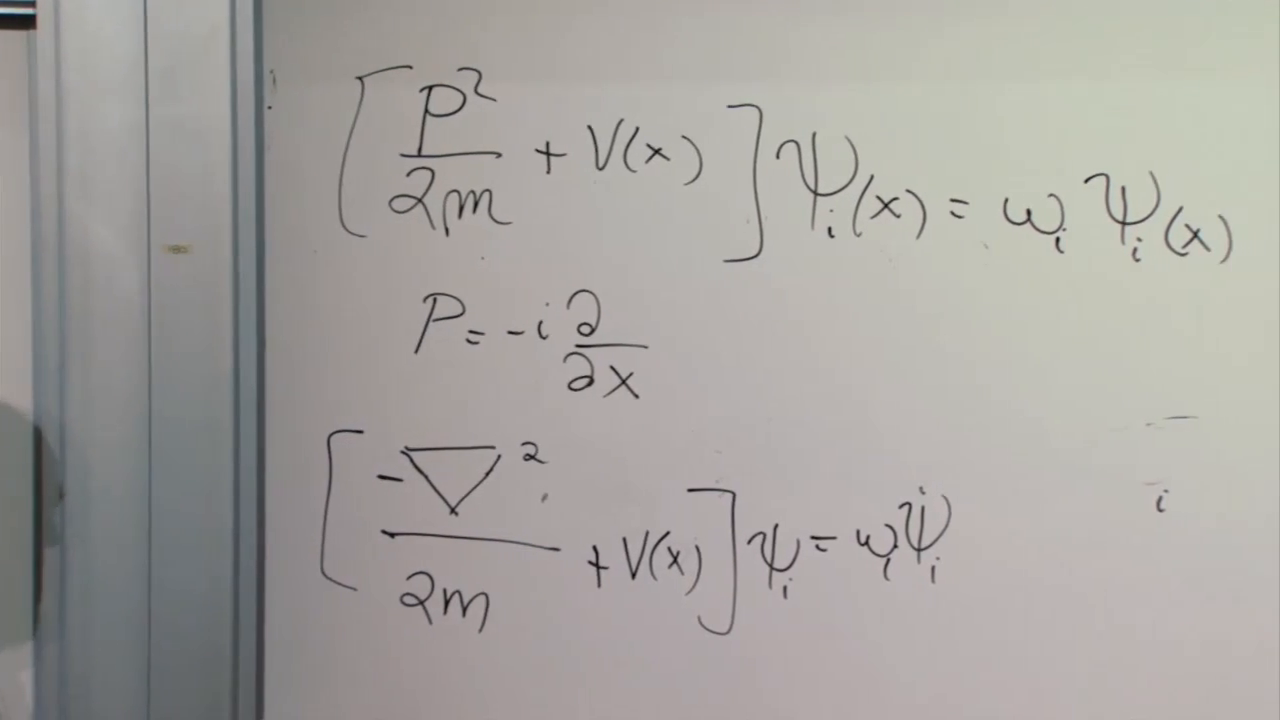
\includegraphics[width=0.94\linewidth]{lecture_07_frame_02.png}
\caption{الانتقال على اللوح من \(p^2/(2m)+V(x)\) إلى الصيغة التفاضلية لمعادلة القيم الذاتية لشرودنغر لجسيم واحد. والمعادلة~\eqref{eq:l07-schrodinger-eigenvalue} هي إعادة بنائها المنقحة.}
\lectureframe{00:54:10}
\end{figure}

بالنسبة إلى دالة موجة مطبَّعة اعتباطية لجسيم واحد، فإن قيمة التوقع المألوفة هي
\begin{equation}
\langle h\rangle_\psi
=\int dx\,\psi^*(x)h\psi(x).
\label{eq:l07-one-particle-energy-expectation}
\end{equation}
وتُستوحى الصيغة عديدة الجسيمات من استبدال دالة الموجة المكتوبة بحرف صغير بالحقل ذي القيم المؤثرية. وهذا ليس برهانًا بعد؛ بل هو التخمين الذي نختبر الآن صحته:
\begin{equation}
H=\int dx\,\Psi^\dagger(x)h\Psi(x).
\label{eq:l07-field-hamiltonian}
\end{equation}

\section{إعطاء الجواب أولًا ثم إثباته}

أدرِج المعادلة~\eqref{eq:l07-field-expansion} في الهاملتوني المقترح:
\begin{align}
\int dx\,\Psi^\dagger h\Psi
&=\int dx
\left(\sum_i a_i^\dagger\psi_i^*(x)\right)
h\left(\sum_j a_j\psi_j(x)\right) \\
&=\sum_{i,j}a_i^\dagger a_j
\int dx\,\psi_i^*(x)h\psi_j(x).
\label{eq:l07-h-expanded}
\end{align}
يؤثر المؤثر التفاضلي \(h\) في دالة الموجة \(\psi_j(x)\) المعتمدة على \(x\)، لا في مؤثر النمط \(a_j\). وبحسب معادلة شرودنغر،
\begin{equation}
h\psi_j(x)=\omega_j\psi_j(x).
\end{equation}
ومن ثم،
\begin{align}
\int dx\,\Psi^\dagger h\Psi
&=\sum_{i,j}a_i^\dagger a_j\omega_j
\int dx\,\psi_i^*(x)\psi_j(x) \\
&=\sum_{i,j}a_i^\dagger a_j\omega_j\delta_{ij} \\
&=\sum_j\omega_j a_j^\dagger a_j.
\label{eq:l07-h-proof}
\end{align}
وهذا يطابق تمامًا المعادلة~\eqref{eq:l07-mode-hamiltonian}. فالتعبير الحقلي الموضعي ومجموع جميع طاقات الجسيمات هما المؤثر نفسه.

\begin{figure}[htbp]
\centering
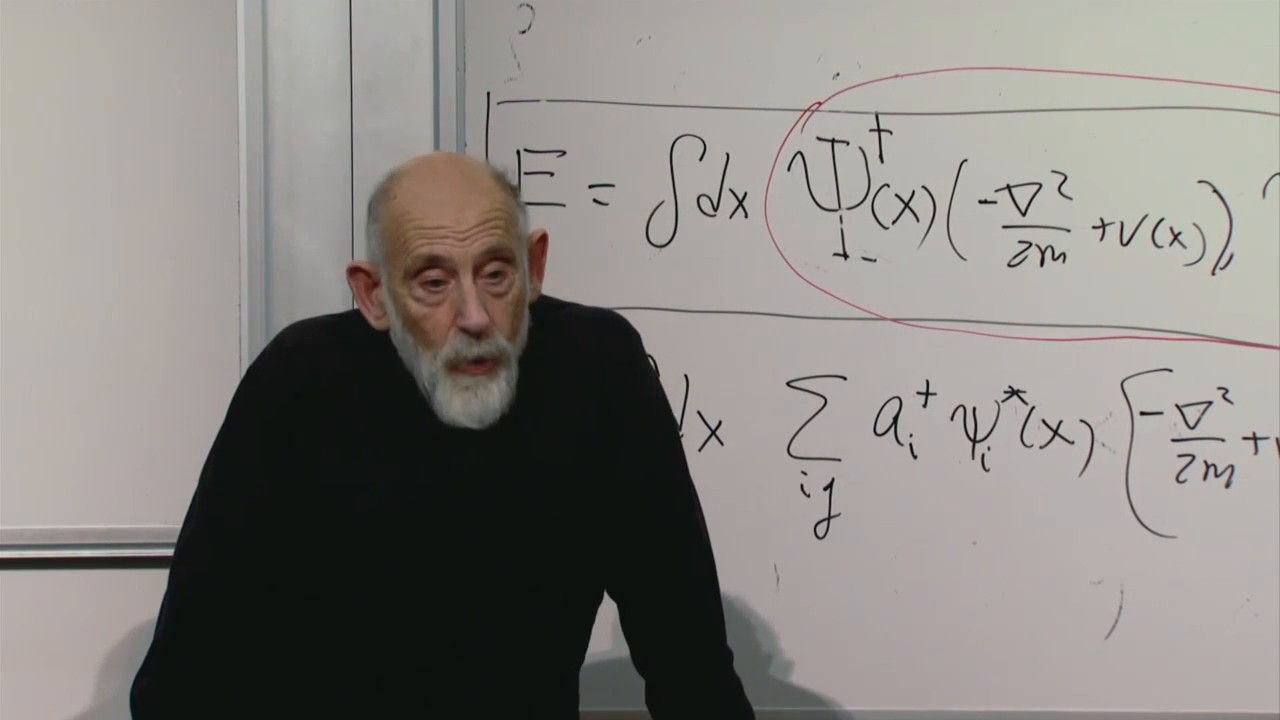
\includegraphics[width=0.94\linewidth]{lecture_07_frame_03.png}
\caption{الهاملتوني الحقلي الذي جرى التأكيد عليه على اللوح، ويبدأ أسفله البرهان بتوسيع الأنماط. وقد أُبقيت الصورة الحية بوصفها شاهدًا؛ وتستعيد المعادلات~\eqref{eq:l07-field-hamiltonian}--\eqref{eq:l07-h-proof} الجبر الكامل.}
\lectureframe{01:05:34}
\end{figure}

لم يُبدَّل ترتيب أي مؤثر خلق مع مؤثر إفناء في هذا الاشتقاق. وقد حُوفظ على ترتيب \(a_i^\dagger a_j\) من البداية إلى النهاية. والأشياء الوحيدة التي نُقلت بحرية هي دوال الموجة من نوع \(c\) وقيمها الذاتية.

\section{لماذا يُعد هذا حقلًا}

لماذا نسمّي \(\Psi(x)\) حقلًا؟ لأنه كمية ذات قيم مؤثرية معرّفة عند كل نقطة من الفضاء، ولأن التراكيب الهرميتية أو المقادير الثنائية الخطية المبنية منه هي مرصودات موضعية. وتمثل الكثافة \(n(x)\) وتعبير الطاقة الموضعي أدناه مثالين. ولا يوجد اختبار رياضي إضافي مخبوء وراء هذه الكلمة.

هذا الحقل ليس الحقل الكهرومغناطيسي. فهو يصف أي نوع غير نسبي تُستمد منه أنماط الجسيم الواحد والهاملتوني \(p^2/(2m)+V\): مثل الذرات البطيئة الحركة، أو النيوترونات، أو البروتونات، أو الإلكترونات. وهذه الجسيمات هي كمّات حقلها الموافق، بالمعنى البنيوي نفسه الذي تكون فيه الفوتونات كمّات الحقل الكهرومغناطيسي.

\begin{classroomqa}
\lecturetimestamp{01:02:45}
\audiencequestion{أين، عند الانتقال من المنظومة عديدة الجسيمات إلى الصيغة أعلاه، دخل الحقل؟}
\lecturerresponse{لقد دخل في المعادلة~\eqref{eq:l07-field-expansion}: فـ \(\Psi(x)\) مؤثر عند كل نقطة مكانية. وتبيّن الاشتقاقات اللاحقة أن جداءاته الموضعية تقيس كثافتي الجسيمات والطاقة. والاعتماد على الموضع مع المحتوى المؤثري هو بالضبط البنية الحقلية التي يجري بناؤها.}
\end{classroomqa}

\section{كثافة الطاقة الموضعية}

تكتب المعادلة~\eqref{eq:l07-field-hamiltonian} الطاقة الكلية على أنها تكامل على الفضاء،
\begin{equation}
\begin{aligned}
H&=\int dx\,\mathcal H(x),\\
\mathcal H(x)
&=-\frac{1}{2m}\Psi^\dagger(x)\nabla^2\Psi(x)\\
&\quad+V(x)\Psi^\dagger(x)\Psi(x).
\end{aligned}
\label{eq:l07-hamiltonian-density}
\end{equation}
والكمية تحت إشارة التكامل هي كثافة طاقة موضعية طبيعية لهذا الهاملتوني. وصيغتها الموضعية غير وحيدة. فعلى سبيل المثال، يستبدل التكامل بالأجزاء الحد الحركي بـ
\begin{equation}
\mathcal H_{\rm kin}(x)
=\frac{1}{2m}\nabla\Psi^\dagger(x)\mathbin{\cdot}\nabla\Psi(x)
\label{eq:l07-kinetic-density}
\end{equation}
حتى حدّ حدودي. ويعطي التعبيران الهاملتوني الكلي نفسه تحت الشروط الحدية المعتادة. وهذا هو الالتباس الصغير المذكور في المحاضرة.

\begin{classroomqa}
\lecturetimestamp{01:05:57}
\audiencequestion{هل يجب تكامل كثافة الطاقة على الفضاء كله؟}
\lecturerresponse{إن التكامل على الفضاء كله يعطي الطاقة الكلية. أما التكامل على منطقة أصغر فيعطي الطاقة المسندة إلى تلك المنطقة، مع مراعاة الالتباس المعتاد في اختيار كثافة موضعية يكون تكاملها الكامل هو الهاملتوني نفسه.}
\end{classroomqa}

\begin{classroomqa}
\lecturetimestamp{01:06:25}
\audiencequestion{كيف يختلف \(N_i\) ذو الحرف الكبير في صيغة الطاقة عن \(n_i\) ذي الحرف الصغير؟}
\lecturerresponse{\(N_i=a_i^\dagger a_i\) مؤثر. والعدد الصحيح \(n_i\) هو إحدى قيمه الذاتية على حالة عدد الإشغال. تؤثر المؤثرات في الحالات؛ أما قيمها الذاتية فهي أعداد عادية.}
\end{classroomqa}

\begin{classroomqa}
\lecturetimestamp{01:06:46}
\audiencequestion{هل يمكن كتابة هاملتوني الحقل نفسه على صورة برا أو كيت في ترميز ديراك؟}
\lecturerresponse{لا. تدل البرا والكيت على متجهات الحالة ومزدوجاتها. الحقل والهاملتوني مؤثران يؤثران في تلك الحالات. وقيمة التوقع مثل \(\langle\Phi|H|\Phi\rangle\) تستخدم كلا النوعين من الكائنات ولا يجوز اعتبارهما شيئًا واحدًا.}
\end{classroomqa}

\section{استعادة الجسيم الواحد والاقتراب من حقل كلاسيكي}

تتضمن الصياغة الموسعة ميكانيكا الكم العادية لجسيم واحد. نقصر فضاء فوك على الحالات التي تحقق
\begin{equation}
N|\Phi\rangle=|\Phi\rangle.
\end{equation}
ضمن ذلك القطاع، يعيد البناء الحقلي إنتاج كل حالة لجسيم واحد وكل تنبؤ خاص بجسيم واحد. لم نستبدل النظرية القديمة؛ بل أدرجناها في فضاء يستطيع أيضًا وصف انعدام الجسيمات، أو جسيمين، أو عدد اعتباطي من الجسيمات.

وعلى الطرف الآخر، يمكن لنمط يشغله عدد كبير جدًا من البوزونات أن يسلك تقريبًا كموجة كلاسيكية. في حالات متماسكة أو شبه كلاسيكية مناسبة، فإن قيمة التوقع
\begin{equation}
\Phi_{\rm cl}(x,t)=\langle\Psi(x,t)\rangle
\end{equation}
تطيع المعادلة ذات المظهر الكلاسيكي
\begin{equation}
i\partial_t\Phi_{\rm cl}(x,t)
=\left(-\frac{\nabla^2}{2m}+V(x)\right)\Phi_{\rm cl}(x,t)
\label{eq:l07-classical-schrodinger}
\end{equation}
في النظرية الحرة غير النسبية. تذكر المحاضرة هذه الصلة بدلًا من اشتقاقها. وهي الجسر بين مجموعة من الكوانتا وحقل موجي: فالإشغالات الكبيرة تقمع التقلبات النسبية وتجعل قيم التوقع المناسبة تسلك سلوكًا كلاسيكيًا.

ولذلك فهذه الصياغة تؤدي دور التنظيم الحسابي كما تؤدي دور الفيزياء. فهي تنظم جميع قطاعات عدد الجسيمات، لكنها تلتقط أيضًا التداخل والتشابك ونشوء الموجات الكلاسيكية من الجسيمات الكمومية.

\begin{classroomqa}
\lecturetimestamp{01:10:43}
\audiencequestion{لماذا يمكن التعامل مع مؤثرات الخلق والفناء داخل التكامل تقريبًا كما لو كانت أعدادًا عادية؟}
\lecturerresponse{لأنه لم يُبدَّل موضع بعضها مع بعض أصلًا. دوال الأنماط العادية تبدّل معها، والمشتقات تؤثر في تلك الدوال فقط. أما تمرير مؤثر فناء عبر مؤثر خلق فيستلزم المبدل وقد يضيف حدًا؛ ولا شيء في البرهان يقوم بهذه الخطوة.}
\end{classroomqa}

\section{استطراد في ترميز ديراك}

بعض هذا الالتباس تاريخي. فدالة الموجة لجسيم واحد تحقق معادلة موجية وتبدو ظاهريًا كحقل كلاسيكي، ومع ذلك فهي أيضًا سعة احتمال. وكان على نظرية الكم المبكرة أن تفصل بين هذين الدورين ثم تشرح كيف تتكون الحقول الموجية القابلة للقياس فعلًا، مثل الكهرومغناطيسية، من كوانتا. ويحل فضاء فوك والحقول ذات القيم المؤثرية هذا التعارض الظاهري.

يجعل ترميز ديراك هذا الفصل موجزًا على نحو غير مألوف. فالكيت ينتمي إلى فضاء متجهي، والبرا إلى فضائه المزدوج، وتجاورهما يشكل جداءً داخليًا. وعندئذ تكاد الصيغة
\begin{equation}
\sum_i|i\rangle\langle i|=\mathbf 1
\end{equation}
تشرح نفسها بنفسها. وتوضح المحاضرة ذلك بحكاية من تدريس ميكانيكا الكم لعلماء الرياضيات: فقد كان المحتوى الرياضي مألوفًا من قبل، لكن الترميز جعل التلاعبات الروتينية شديدة الوضوح إلى درجة أن البنية بدت جديدة. وليست الفكرة أن أحد التخصصين كان يفتقر إلى المفهوم. بل إن ترميزًا حسن الاختيار يمكن أن يجعل العمليات المسموح بها عسيرة الالتباس.

لهذا الدرس أهمية هنا. توجد الآن عدة مؤثرات متميزة:
\begin{itemize}
\item \(h\) يؤثر في دوال الموجة لجسيم واحد بوصفه مؤثرًا تفاضليًا؛
\item \(a_i\) و\(a_i^\dagger\) يعملان على حالات أعداد الإشغال في فضاء فوك؛
\item \(\Psi(x)\) و\(\Psi^\dagger(x)\) و\(N\) و\(H\) تعمل أيضًا على فضاء فوك.
\end{itemize}
يربط التوسع في المعادلة~\eqref{eq:l07-field-expansion} بين السياقين الأولين من غير أن يدمجهما.

\begin{classroomqa}
\lecturetimestamp{01:18:16}
\audiencequestion{هل الحقول مجرد صياغة لوصف مجموعات من الجسيمات؟}
\lecturerresponse{إنها صياغة، لكنها ليست صياغة فارغة. يمكن قياس مراصدها الموضعية، والجسيمات فيها جسيمات كمومية لها تداخل وتشابك، لا حبيبات كلاسيكية. ومؤثرات الحقل تشفِّر بدقة تلك الخواص الجمعية القابلة للقياس.}
\end{classroomqa}

\section{تنبيه متعلق بالنسبية واستطراد كهرومغناطيسي}

البناء حتى الآن غير نسبي. يظل الزخم وسمًا جيدًا للجسيم في الفيزياء النسبية، لكن موضع الجسيم المحدد بحدة مسألة أدق بكثير. وبناءً على ذلك، فإن كثافة عدد الفوتونات الموضعية ليست عمومًا مقدارًا واضح التعريف بقدر \(n(x)\) في النظرية غير النسبية. وتبقى كثافة الطاقة محددة تحديدًا جيدًا، وهي المرصود الموضعي الأكثر أمانًا.

تقدم المحاضرة تشبيهًا كهرومغناطيسيًا مفيدًا، واسترشاديًا على نحو صريح. نجمع المجالين الكهربائي والمغناطيسي في المتجه المركب
\begin{equation}
\mathbf F=\mathbf E+i\mathbf B,
\qquad
\mathbf F^*=\mathbf E-i\mathbf B.
\label{eq:l07-riemann-silberstein}
\end{equation}
وعندئذ
\begin{equation}
\mathbf F^*\mathbin{\cdot}\mathbf F
=\mathbf E^2+\mathbf B^2,
\label{eq:l07-em-density}
\end{equation}
وهو يتناسب مع كثافة الطاقة الكهرومغناطيسية في الوحدات المتعارف عليها. وهذا ليس حرفيًا كثافة احتمال للفوتون. والأفضل أن يُنظر إليه بوصفه متغيرًا حقليًا مضغوطًا يقيس مربع معياره كثافة الطاقة، أو، على نحو غير رسمي، بوصفه كثافة فوتونات موزونة بطاقة الفوتون.

\begin{classroomqa}
\lecturetimestamp{01:19:10}
\audiencequestion{هل يمكن مطابقة كثافة الفوتونات مع شدة المجال الكهربائي؟}
\lecturerresponse{فقط على نحو نوعي ومع الحذر. بالنسبة إلى الفوتونات النسبية، ليس عدد الجسيمات الموضعي هو المفهوم المفضل. والعبارة الموثوقة هي أن \(E^2+B^2\) يتناسب مع كثافة الطاقة، وأن التركيب المركب \(\mathbf E+i\mathbf B\) يصوغ معادلات ماكسويل في صورة شبيهة بشرودنغر.}
\end{classroomqa}

\begin{classroomqa}
\lecturetimestamp{01:20:09}
\audiencequestion{لماذا يمكن لجسيم نسبي أن يملك زخمًا محددًا بينما يكون الموضع إشكاليًا؟}
\lecturerresponse{لأن الزخم يشكّل وسمًا واضحًا لتمثيلات الجسيم الواحد النسبية، في حين أن التوضع الصارم يتعارض مع خلق الجسيمات ومع الوصف الحقلي النسبي. لا تطور هذه المحاضرة تلك النظرية؛ وإنما يشير هذا التحذير إلى حد تفسير الكثافة غير النسبي الحالي.}
\end{classroomqa}

\section{الترتيب وثابت الحالة القاعية}

لا يمكن تغيير ترتيب المؤثرات على نحو اعتباطي. بالنسبة إلى الأنماط البوزونية،
\begin{equation}
a_i a_i^\dagger=a_i^\dagger a_i+1.
\end{equation}
وبناءً على ذلك، فإن استبدال الترتيب العادي \(\Psi^\dagger h\Psi\) بالترتيب المعكوس \((h\Psi)\Psi^\dagger\)، أو إجراء هذا الاستبدال في نظيره المتكامل على الوجه الصحيح، يضيف مساهمة المبدل. وفي أساس الأنماط يكون هذا مجموعًا إضافيًا مقداره كمّ واحد من الطاقة لكل نمط. وهو ثابت الحالة القاعية أو ثابت طاقة نقطة الصفر، وفي المتصل يحتاج إلى تنظيم. لا تتوسع المحاضرة في هذه المسألة هنا؛ وإنما تنبه فقط إلى أن الترتيبين غير متساويين.

\begin{classroomqa}
\lecturetimestamp{01:22:04}
\audiencequestion{ما الذي يحدث إذا بُدِّل ترتيب \(\Psi\) و\(\Psi^\dagger\) في الهاملتوني؟}
\lecturerresponse{يجب تضمين مبادلهما. لذلك فإن عكس الترتيب يضيف مساهمة في طاقة الحالة القاعية مستقلة عن الحالة بدلًا من إعادة إنتاج التعبير نفسه. ويُبقى الهاملتوني المعروض في الترتيب العادي، \(\Psi^\dagger h\Psi\).}
\end{classroomqa}

\section{الزخم بوصفه الاختبار الأخير}

تعيد الدقائق الأخيرة عملية الترقية نفسها مرة أخرى. بالنسبة إلى جسيم واحد،
\begin{equation}
\langle p\rangle_\psi
=\int dx\,\psi^*(x)\left(-i\partial_x\right)\psi(x).
\label{eq:l07-one-particle-momentum}
\end{equation}
فإن استبدال دالة الموجة بالحقل يعطي مؤثر الزخم الكلي
\begin{equation}
P=\int dx\,\Psi^\dagger(x)\left(-i\partial_x\right)\Psi(x),
\label{eq:l07-field-momentum}
\end{equation}
أو، في ثلاثة أبعاد،
\begin{equation}
\mathbf P=\int d^3x\,\Psi^\dagger(\mathbf x)
\left(-i\boldsymbol\nabla\right)\Psi(\mathbf x).
\end{equation}
تحمل الحقول زخمًا. فالليزر ذو القدرة الكافية ينقل زخمًا إلى جدار ويؤثر بقوة؛ وفي الوصف الكمومي يكون الزخم الذي يحمله الحقل هو مجموع زخوم الفوتونات.

المعادلة~\eqref{eq:l07-field-momentum} تمثل مؤثرًا، لا قيمة توقع. وإذا أُعطيت حالة في فضاء فوك \(|\Phi\rangle\)، أمكن عندئذ حساب
\begin{equation}
\langle P\rangle_\Phi=\langle\Phi|P|\Phi\rangle.
\end{equation}
ويلزم كل من مؤثر وحالة لتكوين قيمة توقع. وإن الخلط بين المرصود ومتوسطه يمحو بالضبط التمييز الذي عملت المحاضرة على إقامته.

\begin{classroomqa}
\lecturetimestamp{01:26:02}
\audiencequestion{هل زخم الحقل المعروض هو بالفعل الزخم المتوسط؟}
\lecturerresponse{لا. إنه المؤثر الهيرميتي الذي يمثل المرصود. وبإعطاء حالة ووضع المؤثر بين براها وكيتها تُحصَل قيمة توقع؛ ومع ذلك يمكن للقياس أن يتقلب حول ذلك المتوسط.}
\end{classroomqa}

هذه هي نقطة التوقف الطبيعية. انطلاقًا من الجسيمات، شيدنا حقول خلق وفناء موضعية، واستخدمناها لعد الجسيمات، وأعدنا كتابة مجموع طاقات الجسيم الواحد وزخومه على صورة مؤثرات حقلية. والخطوة التالية ليست تغييرًا آخر في الترميز. بل هي أن نسمح لمؤثرات الحقل بأن تمثل عمليات فيزيائية: جسيمات تضمحل، وجسيمات تتبعثر، وأنواع الجسيمات تتحول بعضها إلى بعض.
